\chapter{Trust graph}
\label{trust-graph}

When looking into the construction of trust graphs, one can get inspiration from solutions that have worked in human societies for centuries.
In his book "Sapiens: A Brief History of Humankind" \cite{harari2014sapiens}, Yuval Noah Harari, states that the most important feature of human language is rumor; it lets us know which person is or is not trustworthy without having to interact with him/her directly. If our best friend Bob tells us that Charlie is a thief, we do not need to get robbed to be convinced about it. The same applies to an inverse scenario--if Bob tells us that Charlie sells excellent quality products, we are more likely to buy products from him; we are biased towards people about whom we hear positive rumors. Each person we know directly or indirectly gets labeled with some tags. One can be labeled as Helpful, Conscientiousness, or Untrustworthy, while others can be labeled as Unhelpful, Lazy but Trustworthy etc. In this thesis we  limit the scope just to the Trustworthiness dimension.

Suppose we have three friends Alice, Bob, and Charlie. Alice and Bob tell us that David is Trustworthy, while Charlie claims that he is not. The decision to label David as Trustworthy or Untrustworthy requires some decision evaluation algorithm.
One might for example assume that if there is at least one person who does not trust him, there must be something wrong with him and so label him as Untrustworthy. One can use another, majority-based evaluator: if a majority of my friends trust Charlie, so will I. Another one can slightly generalize this evaluator and say that person is trustworthy, only if a given percentage $\xi$ of my friends trust him. 

We now introduce some conventions. A trust relation implies that two nodes trust each other, either by being friends (a friendship relation being given a priori) or have a large enough proportion of mutual friends. 
Let $N$ be a set of all considered individuals. Let $F_n \subset N$ be the set of all $n$'s friends. Then 
\begin{equation}
\%(n_1, n_2) = \frac{|F_{n_1} \cap F_{n_2}|}{|F_{n_1}|}    
\end{equation}
is the proportion of $n_1$'s friends who are also $n_2$'s friends. Let's call $\xi$ (where $0 \le \xi \leq 1$) the minimum value of $\%(n_1, n_2)$ needed to create trust relation from $n_1$ to $n_2$.

Coming back to our example, we trust David only if the majority of our friends trust him. We denote trust function as $T : N \times N \rightarrow \{true, false\}$, $T(n_1,n_2) = \%(n_1,n_2) > \xi$. 
To evaluate if we should create trust relation to David, let $\xi = 0.5$ and assume Alice, Bob and Charlie are our friends, and Alice and Bob are David's friends, but Charlie is not.
\begin{equation}
\begin{split}
T(Me, David) &= \%(Me, David) > \xi \\
&= \frac{|F_{me} \cap F_{David}|}{|F_{me}|} > \xi \\
&= \frac{2}{3} > \frac{1}{2}
\end{split}
\end{equation}
Then David is \textbf{Trustworthy} and we should create trust relation to him.

Intuitively, people with low $\xi$ easily get manipulated and can be called naive; people with high $\xi$ hardly get convinced and can be called stubborn. 

Having a trust model, we can describe an algorithm to generate a trust graph.
\begin{enumerate}
    \item start with initial $N_0$ nodes and $E_0$ edges and connect them randomly, such that the graph is connected.
    \item each remaining node $n \in N \backslash N_0$, gets connected to one randomly selected node.
    \item for each node $n \in N$,

\quad for each node $f \in F_n$,

\quad \quad for each node $p \in F_f \backslash F_n$,

\quad \quad \quad if $T(n, p) = true$, add connection between $n$ and $p$.
\end{enumerate}

We find some similarities between our graph generator and a trust network formed in PGP systems \cite{RFC4880O31:online} (with just one level of indirect trust); therefore, we call this algorithm the Web of Trust generator.

In Fig. \ref{fig:trustgraph500} we see the resulting trust graph for $N=500$, $N_0=10$, $E_0=20$ and $\xi = 0.5$, and its corresponding histogram of node degree in Fig. \ref{fig:trustgraph500histogram}

\begin{figure}[h!]
    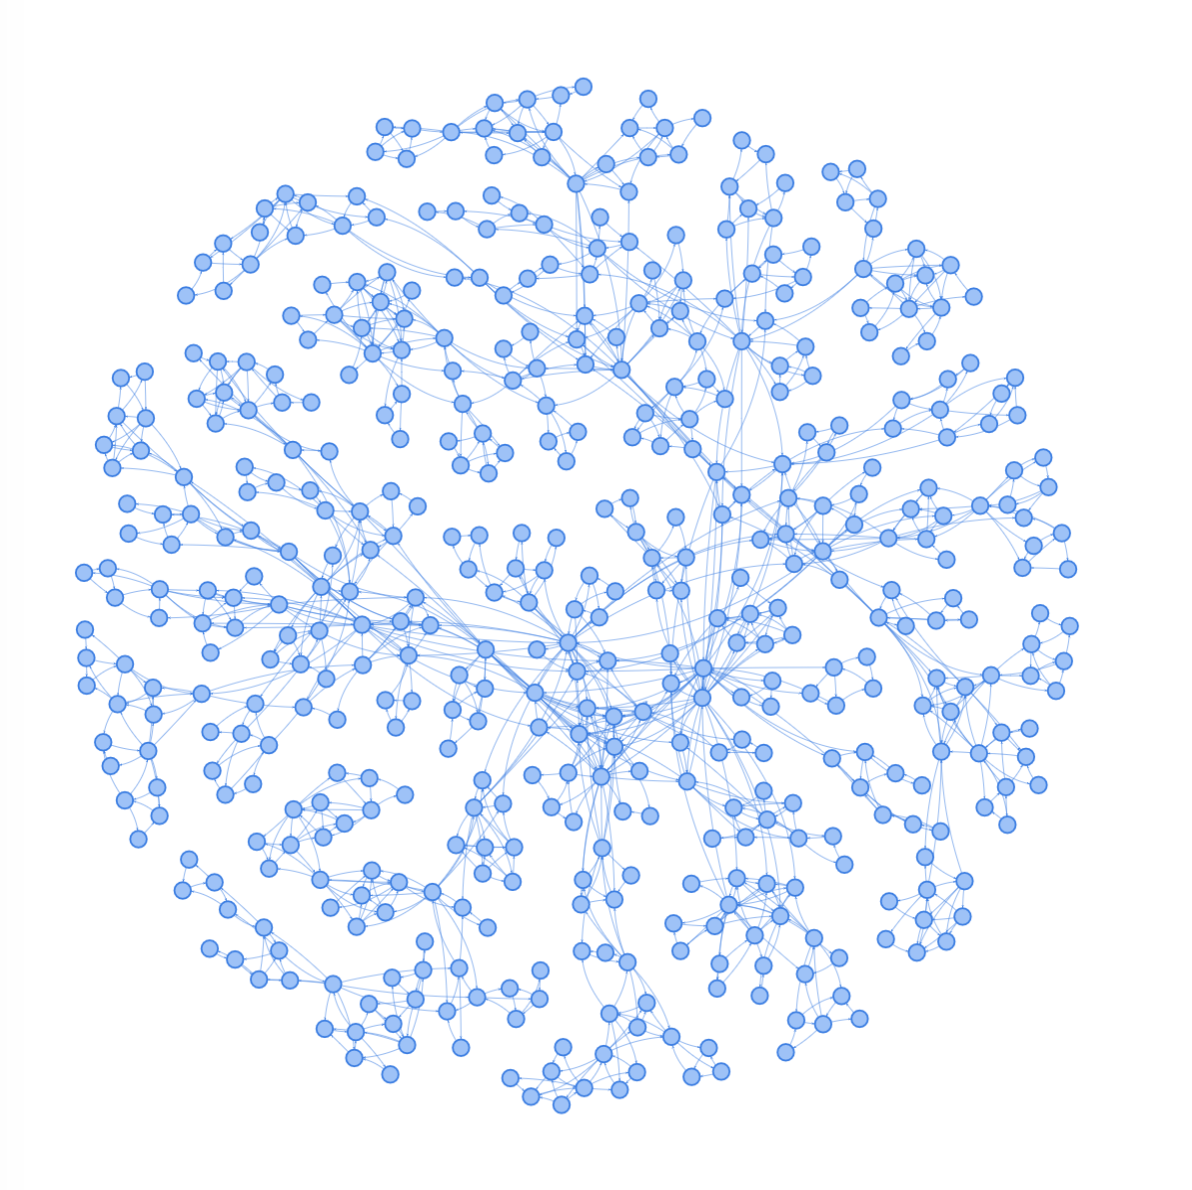
\includegraphics[width=\textwidth]{img/webOfTrust500Graph.png}
    \centering
    \caption{Trust Graph generated by Web Of Trust algorithm for $N=500$, $N_0=10$, $E_0=20$ and $\xi = 0.5$}
    \label{fig:trustgraph500}
\end{figure}

\begin{figure}[h!]
    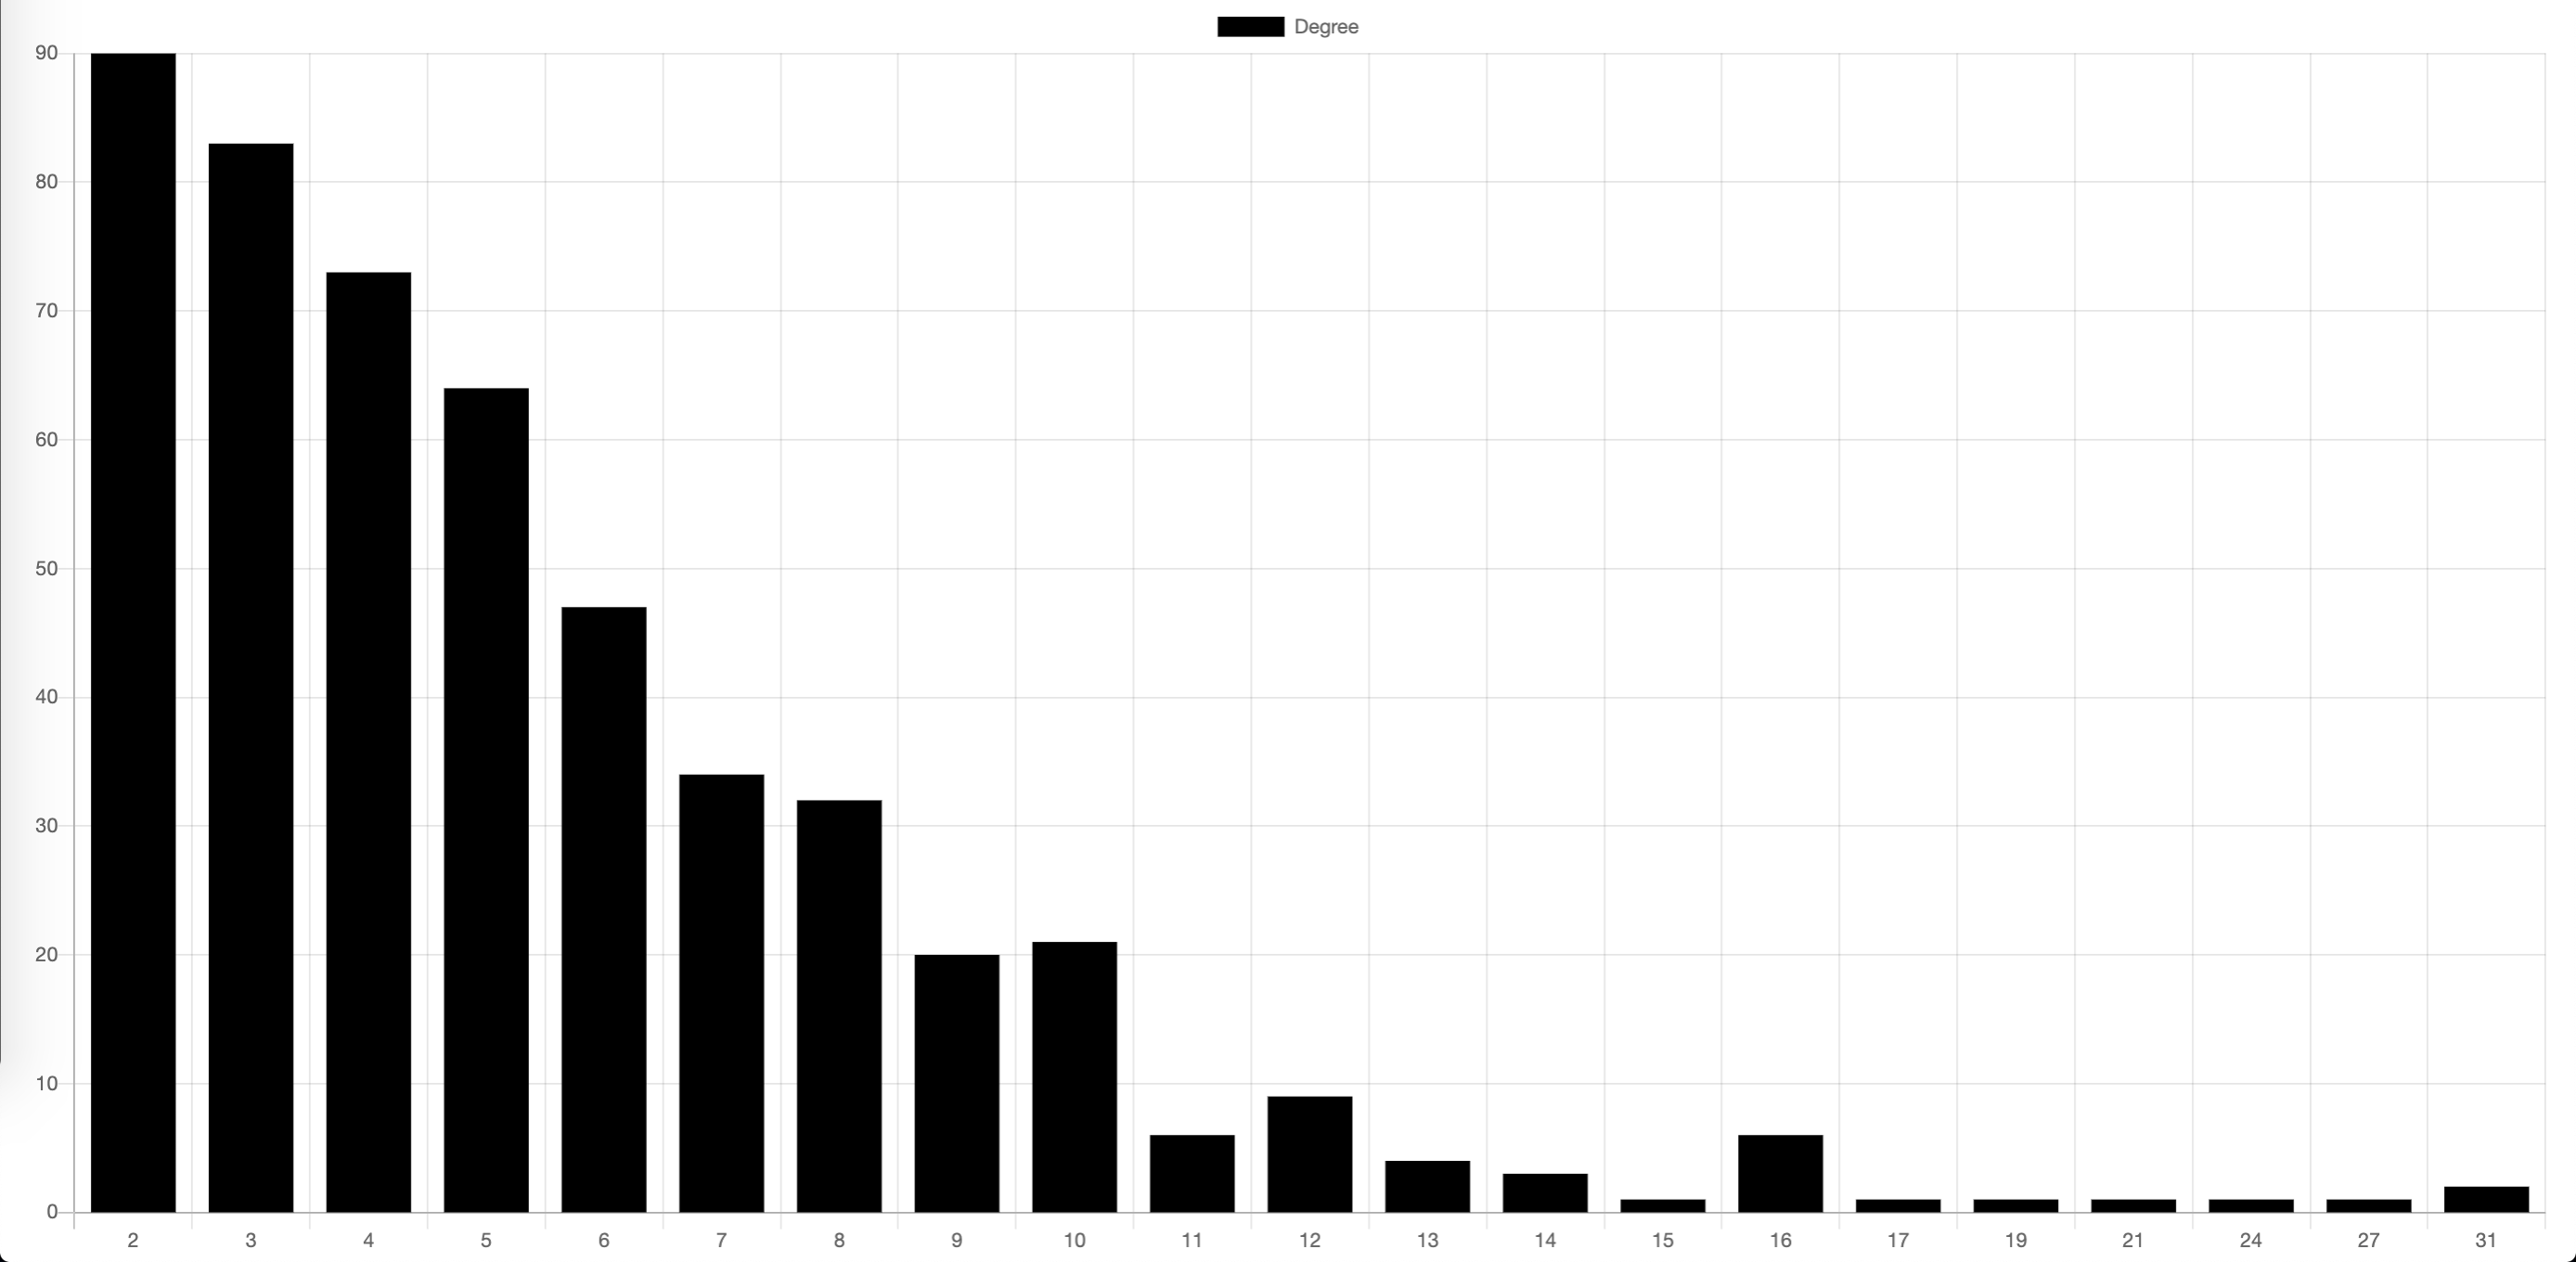
\includegraphics[width=\textwidth]{img/webOfTrust500Hist.png}
    \centering
    \caption{Degree histogram generated by Web Of Trust algorithm for $N=500$, $N_0=10$, $E_0=20$ and $\xi = 0.5$}
    \label{fig:trustgraph500histogram}
\end{figure} 

\section{Other trust graph generators}

\paragraph{Probabilistic duplication}
Another trust graph generator used in \cite{konorski2019mitigating} is based on probabilistic duplication and works as follows:
\begin{enumerate}
    \item start with initial $N_0$ nodes and $E_0$ edges and connect them randomly, such that the graph is connected
    \item add new node $n_1$ and connect it to one randomly selected node $n_2$ in the current graph.
    \item connect $n_1$ to $n_2$'s friends, to each with probability $\phi$. Repeat steps 2 and 3 $|N \backslash N_0|$ times. 
\end{enumerate}

The most important advantage of this generator is the fact that it produces almost scale-free graphs. Figure \ref{fig:propdup500graph} shows the graph generated by this method and Figure \ref{fig:propdup500histogram} shows the histogram of node degree.

\begin{figure}[h!]
    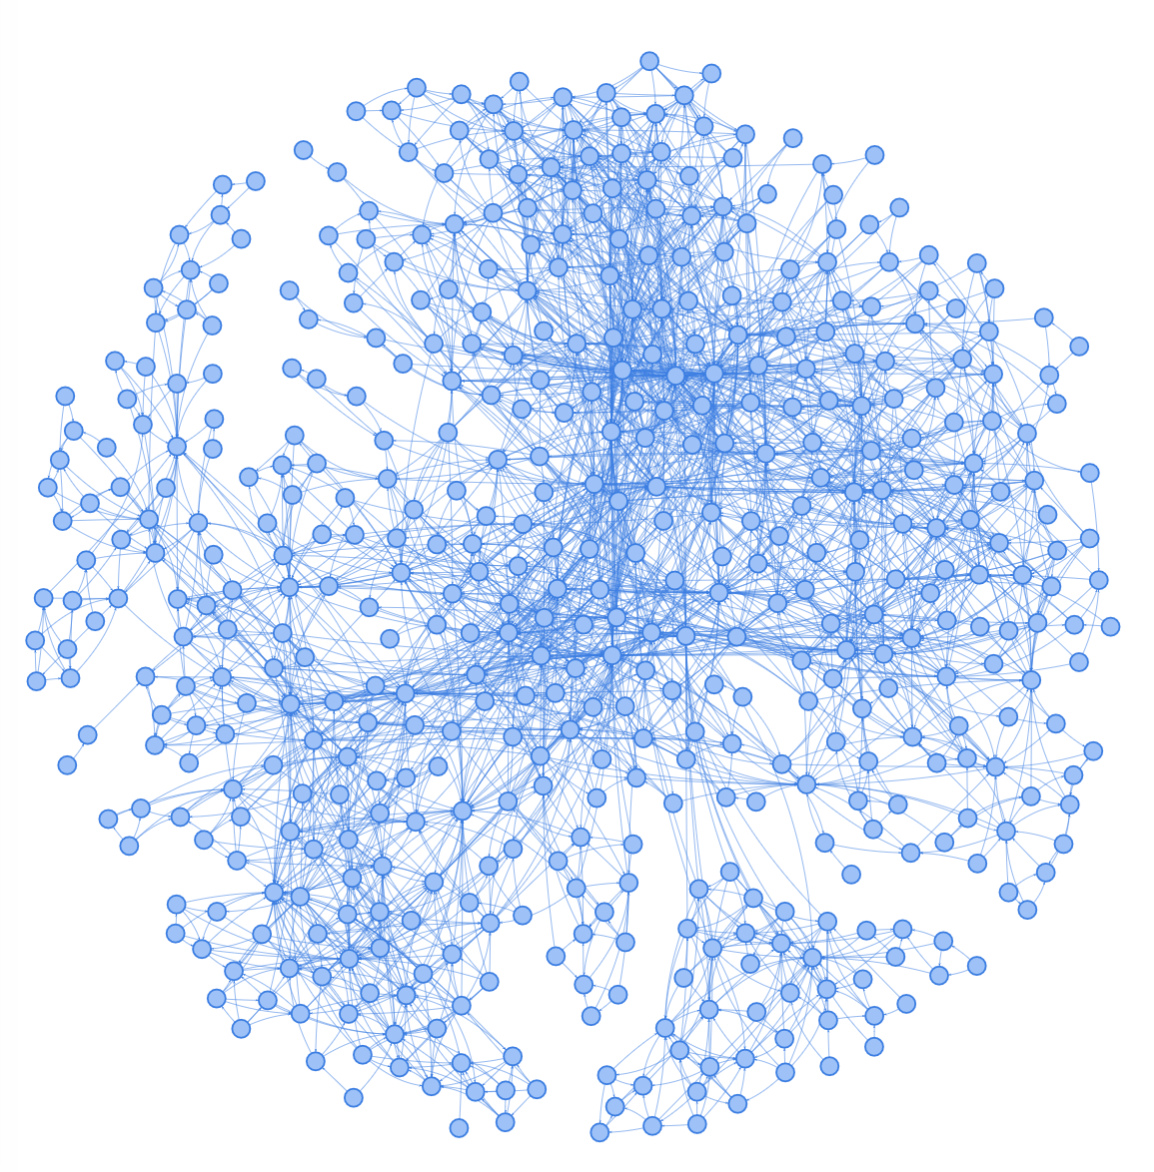
\includegraphics[width=\textwidth]{img/propDup500Graph.png}
    \centering
    \caption{Trust Graph generated by Probabilistic Duplication algorithm for $N=500$, $N_0=10$, $E_0=20$ and $\phi = 0.5$}
    \label{fig:propdup500graph}
\end{figure}

\begin{figure}[h!]
    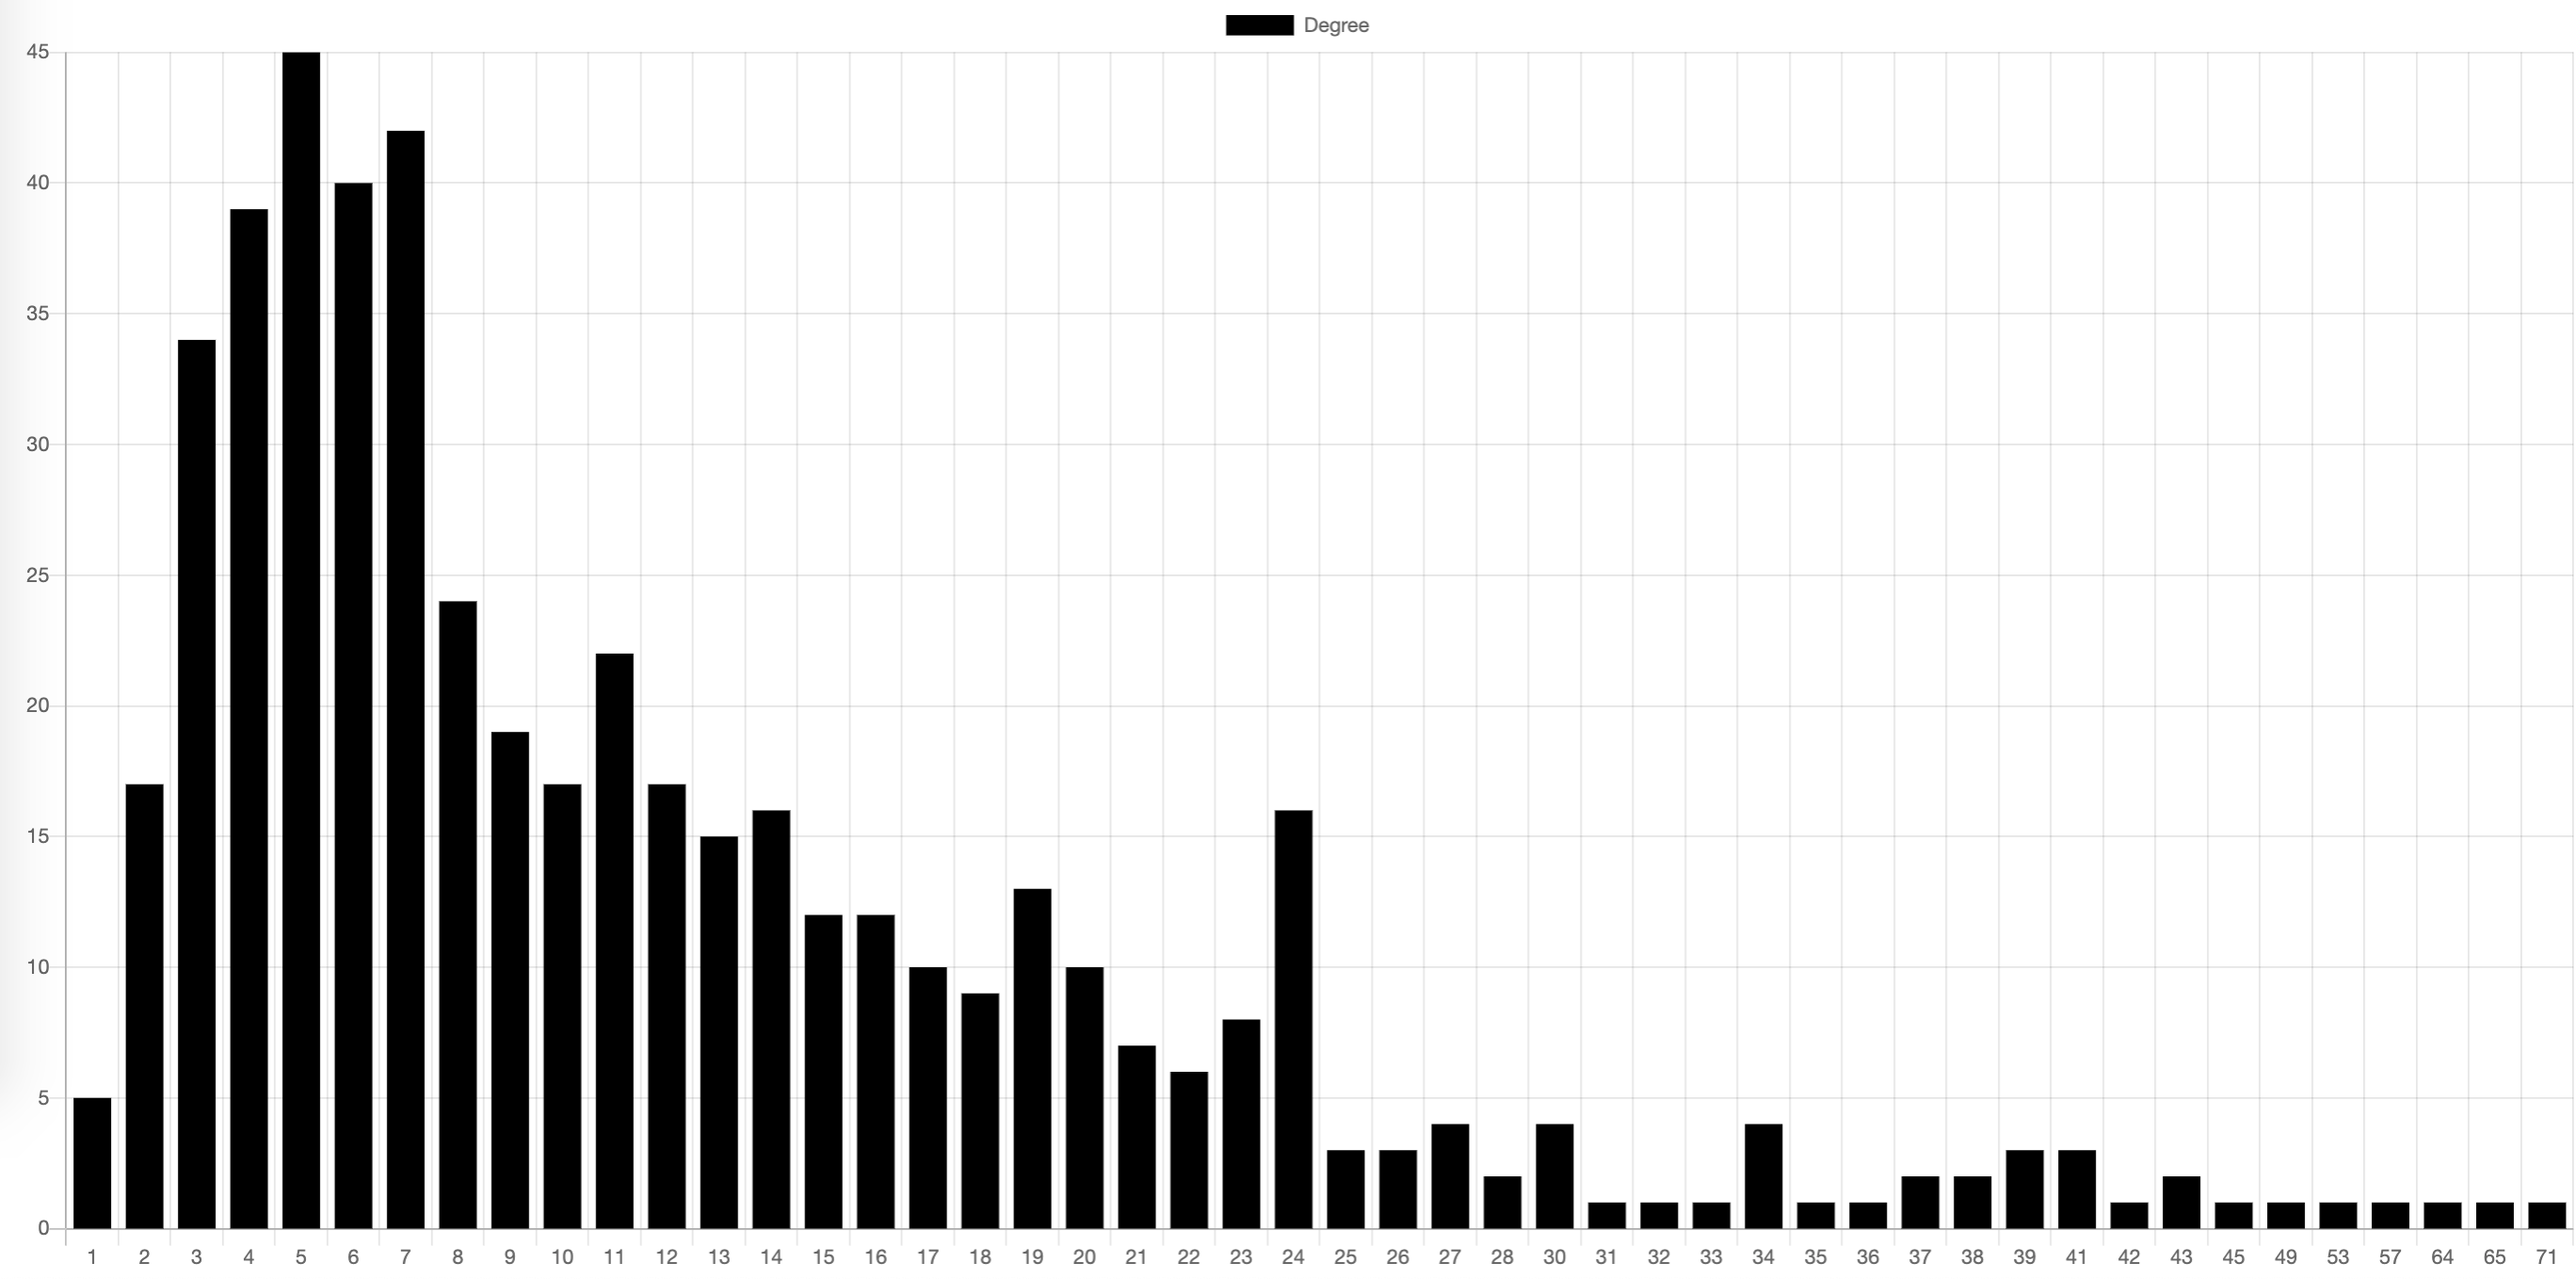
\includegraphics[width=\textwidth]{img/propDup500Hist.png}
    \centering
    \caption{Degree histogram generated by Probabilistic Duplication algorithm for $N=500$, $N_0=10$, $E_0=20$ and $\phi = 0.5$}
    \label{fig:propdup500histogram}
\end{figure} 

\paragraph{Random generator}

A random graph generator is the simplest one. Take $N$ nodes, $E$ edges and connect them randomly, such that the graph is connected. Although random trust graphs are far from  real-world trust graphs, we use it for comparison. Figure \ref{fig:random500graph} shows the graph generated by the method and Figure \ref{fig:random500histogram} shows the histogram of node degree.

\begin{figure}[h!]
    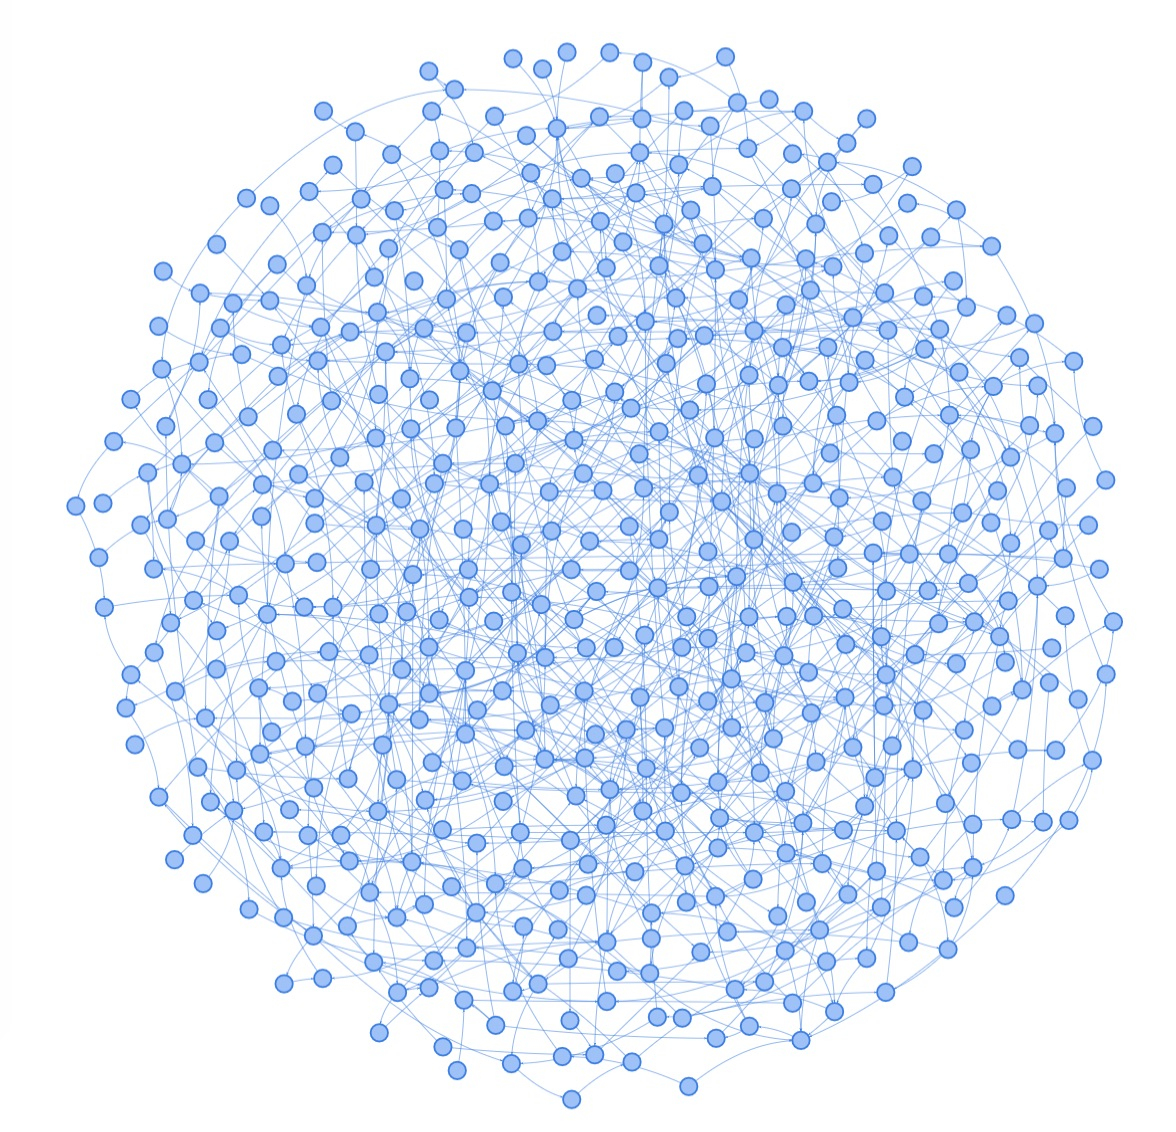
\includegraphics[width=\textwidth]{img/random500Graph.jpg}
    \centering
    \caption{Random graph generated by Random generator for $N=500$ $E=1000$}
    \label{fig:random500graph}
\end{figure}

\begin{figure}[h!]
    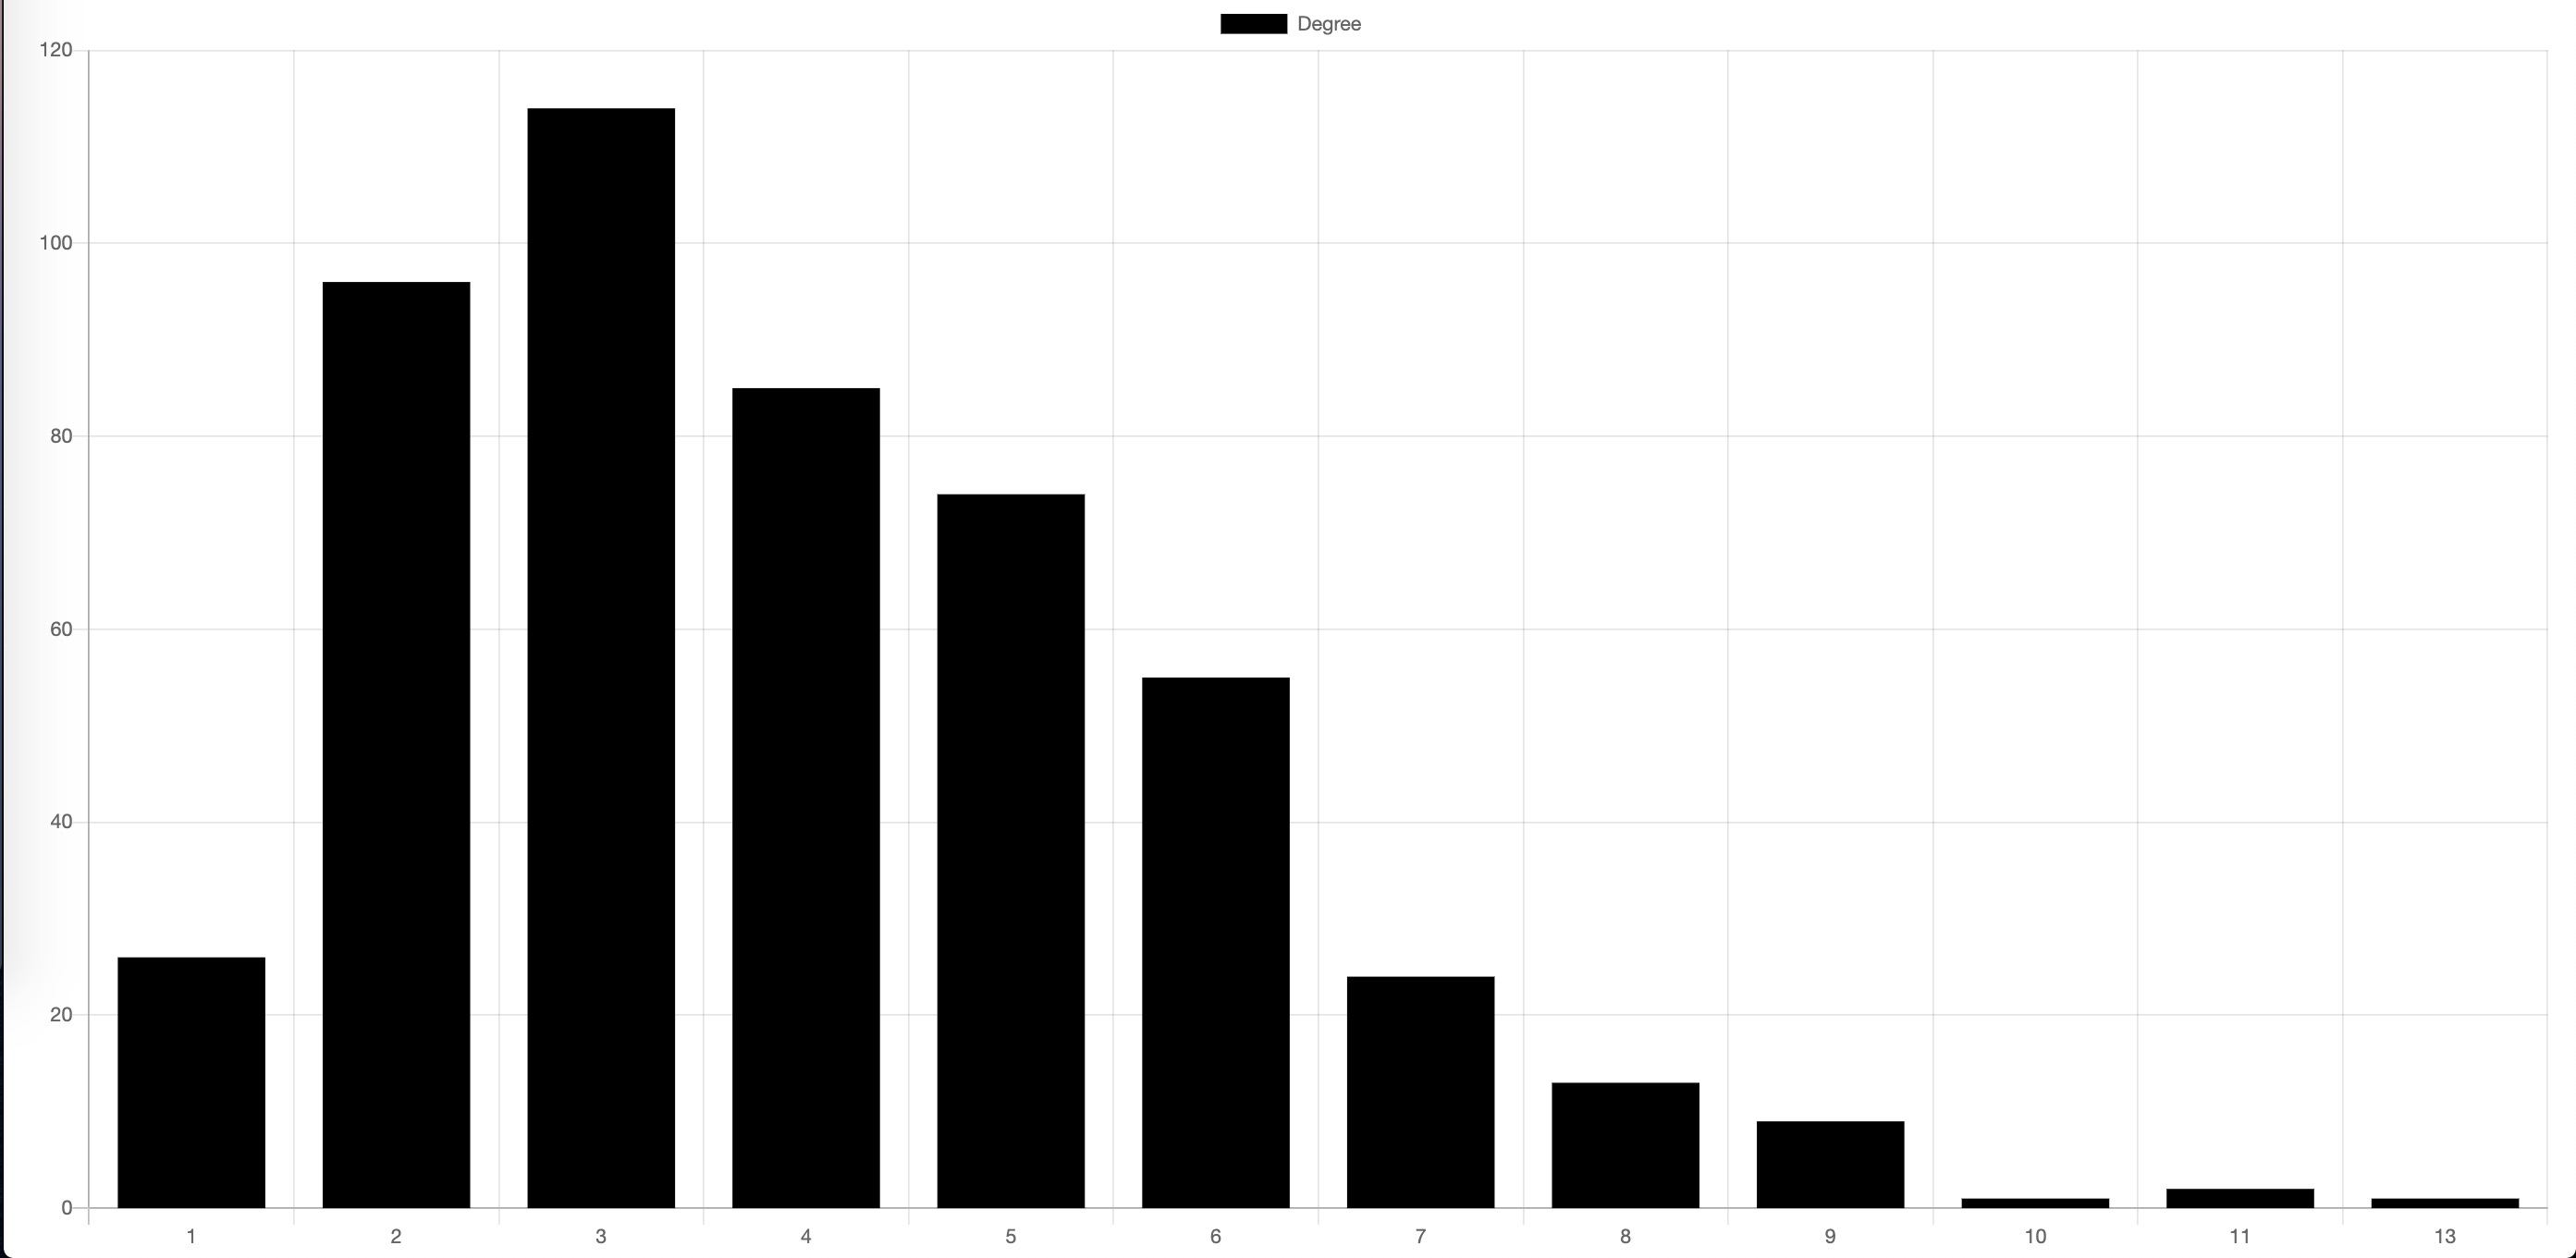
\includegraphics[width=\textwidth]{img/random500Histogram.jpg}
    \centering
    \caption{Degree histogram generated by Random generator for $N=500$ and $E=500$}
    \label{fig:random500histogram}
\end{figure} 